\section{Parte 1: Diagrama de Casos de Uso (UML)}

\subsection{Actores del Sistema}
\begin{itemize}[nosep]
    \item \textbf{Participante (Ciudadano / Servidor):} Consulta cursos, se inscribe con DNI, marca asistencia mediante QR y descarga su certificado digital.
    \item \textbf{Docente (Capacitador):} Genera el código QR dinámico de la sesión, registra calificaciones (0--20) y cierra las actas académicas.
    \item \textbf{Administrador:} Parametriza cursos, cupos, docentes, y genera reportes ejecutivos consolidados.
    \item \textbf{Sistema Central (RENIEC / Hashing):} Valida DNI, controla cupos, genera tokens QR y calcula el hash criptográfico SHA-256 de cada certificado emitido.
\end{itemize}

\subsection{Diagrama de Casos de Uso}
El diagrama modela el límite del sistema (\textit{boundary}) y las relaciones \texttt{<<include>>} y \texttt{<<extend>>}. Archivo nativo editable: \texttt{diagramas/casos\_de\_uso\_sigc.drawio}.

\begin{figure}[H]
    \centering
    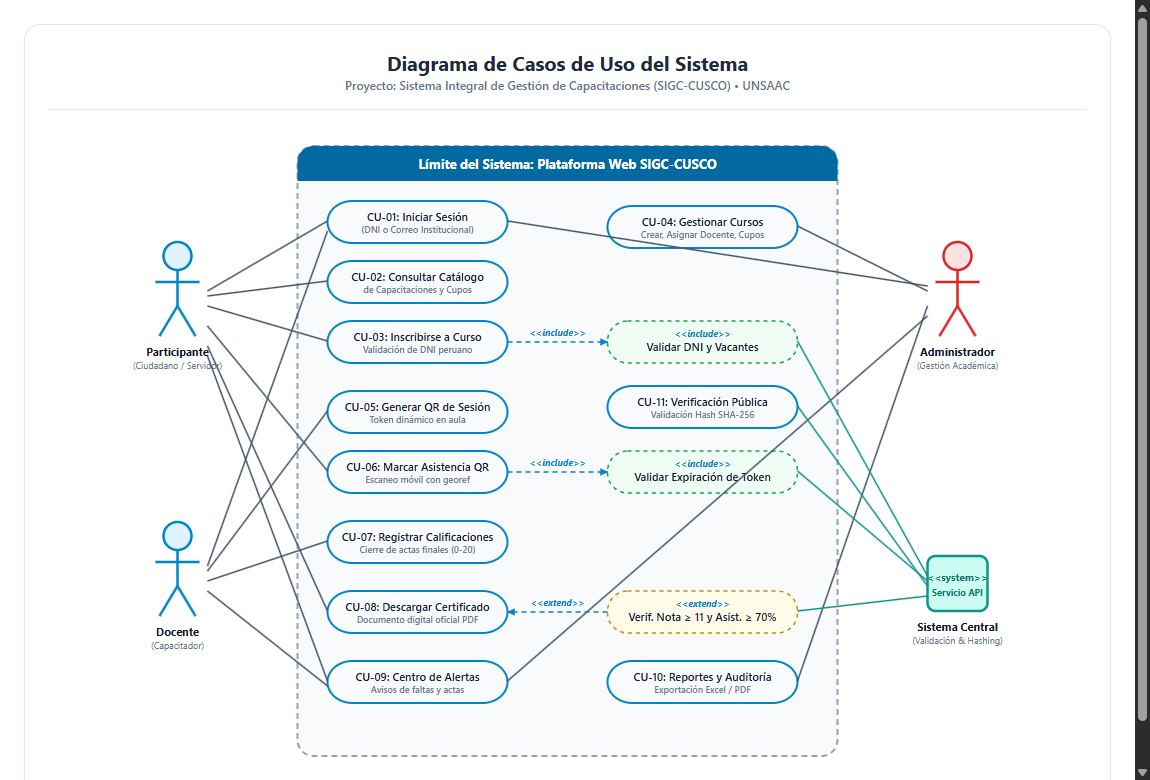
\includegraphics[width=0.98\textwidth]{diagrama_casos_uso.png}
    \caption{Diagrama de Casos de Uso del Sistema SIGC-CUSCO (Draw.io).}
    \label{fig:casos_uso}
\end{figure}

\begin{table}[H]
\centering
\footnotesize
\begin{tabularx}{\textwidth}{l P{3.8cm} P{3.0cm} Y}
\toprule
\textbf{Código} & \textbf{Caso de Uso} & \textbf{Actores} & \textbf{Descripción y Relaciones} \\
\midrule
\textbf{CU-01} & Iniciar Sesión & Todos los usuarios & Autenticación por DNI o correo institucional con RBAC. \\
\textbf{CU-02} & Consultar Catálogo & Participante & Exploración de cursos, vacantes y cronogramas. \\
\textbf{CU-03} & Inscribirse a Curso & Participante & \texttt{<<include>> Validar DNI y Cupos}: Registro inmediato. \\
\textbf{CU-04} & Gestionar Cursos & Administrador & Alta de capacitaciones, horas y asignación de docentes. \\
\textbf{CU-05} & Generar QR de Sesión & Docente & Generación de token dinámico proyectado en aula. \\
\textbf{CU-06} & Marcar Asistencia QR & Participante & \texttt{<<include>> Validar Token}: Escaneo móvil con control horario. \\
\textbf{CU-07} & Registrar Notas y Actas & Docente & Ingreso de calificaciones vigesimales y cierre de actas. \\
\textbf{CU-08} & Descargar Certificado & Participante & \texttt{<<extend>> Requisitos}: Emisión condicionada ($\ge 11$ y $\ge 70\%$ asist.). \\
\textbf{CU-09} & Centro de Alertas & Todos los usuarios & Notificaciones de plazos perentorios, inasistencias y notas. \\
\textbf{CU-10} & Reportes y Auditoría & Administrador & Consolidado estadístico y exportación a PDF y Excel. \\
\textbf{CU-11} & Verificación Pública QR & Sistema / Público & Validación de certificados auténticos vía hash SHA-256. \\
\bottomrule
\end{tabularx}
\caption{Matriz de especificación de Casos de Uso.}
\label{tab:casos_uso}
\end{table}
